\chapter{Digital Video Broadcasting (DVB)}
There are many parts that are needed to provide Digital Video 
Broadcasting (DVB) with a secure way of transmitting streams of data 
without facing the risk of content getting stolen. The following parts 
will be treated in this thesis:

\begin{itemize}
\item Head-end - explained in section \ref{sec:HE}
\item CAS - explained in section \ref{sec:CAS}
\item Common Interface - explained in section \ref{sec:CI}
\item Scrambler - explained in chapter \ref{ch:Scrambling}
\item Descrambler - the inverse of a scrambler.
\end{itemize}

%% \section{Head-end}
%% The head-end is the part where the scrambler is located. Among other 
%% things present on the head-end are decoders and generation of program
%% specific information. Content providers send their programs to the 
%% head-end, where the content is decoded, encrypted and then passed on.

\section{Control word} \label{sec:setup}
\emph{Transport Stream}s (TS) which contains data received from 
distributors are scrambled using a key which is called a 
\emph{control word}. Although the control word is required to be changed
every 120th second, it is common to change it as often as every 
10th seconds. Finding out just one control word has very little effect, 
since it will only be usable for a few seconds before it is changed. 
The high frequency in which the control words are changed thereby 
provides the system with security. The control word is generated 
randomly to make sure that consecutive control words are not related 
to each other.

The control word is sent to a \emph{Conditional Access System} (CAS) 
where the control word is encrypted as an 
\emph{Entitlement Control Message} (ECM). The CAS also generates an 
\emph{Entitlement Management Message} (EMM) which tells the smart-card 
what contents the user is allowed access to. This could for instance 
be whether the user has paid to view premium football games or not.
The ECM and EMM are then sent back to the head-end where they are 
attached to the scrambled TS packet using a multiplexer. 
This package is sent to a receiver, which is usually a TV. The ECM, 
EMM and TS are separated when they arrive. The ECM and TS packet are 
sent through a \emph{Common Interface} (CI) to a \emph{Conditional 
Access Module} (CAM), where the ECM (previous control word) is 
decrypted using a decryption algorithm located on a smart card. 
The resulting control word is then used to descramble the TS packet. 
The TS packet is encrypted once more if the CI is a CI-Plus, otherwise 
it is sent in the clear back to the receiver where the data is 
processed before it is dispatched to the user. The CI and CI-Plus as 
well as the extra encryption are all discussed in section \ref{sec:CI}.

\section{Conditional Access System} \label{sec:CAS}
\emph{Conditional Access} (CA) is used to make sure that a user 
fulfills an amount of criteria before being able to view content. A 
Conditional Access System (CAS) consists of an EMM-generator and an 
ECM-generator among others. An ECM-generator is basically an encryption 
of the control word. The algorithms used in generators differ between 
CA systems and is kept very secret, to make sure that the control word 
can not be stolen during transmission.

The ECM is generated using the control word, while the EMM is generated 
based on subscription- and payment information related to the user. The 
EMM can allow things, stretching from allowing a user to view a video 
for a few hours, to access a certain channel for an extended period of 
time. A TV will not broadcast any channels without receiving an EMM 
allowing it to.
\Warning[Source]{You need to find more sources than just Patrik}

An example is that a user needs to pay for TV-services to be able 
to access content. The CA system generates an EMM which tells 
the smart-card whether the user is allowed to access the requested 
material or not. The content provider also generates an ECM based on 
the control word, which the smart-card decrypts and passes to the 
descrambler, to decrypt the video stream. This is done if the EMM 
allows it.

\subsection{Standards}
Some of the CA systems currently in use are Viaccess, Conax, Irdeto, NDS, Strong 
and NagraVision. There are different \emph{Conditional Access Module}s (CAM) 
that are used, and which one is needed depends on the content provider. NDS is 
used by Viasat, Conax is used by Com Hem, Viaccess is used by Boxer and Strong 
is used by Canal Digital for instance.

\begin{longtable}{| l | c | c |}
  \hline
  CA system & Used by & Supports CI+ \\ \hline
  
  Viaccess & Boxer, SVT & Yes \\ \hline
  Conax & Com Hem & Yes \\ \hline
  Strong & Canal Digital & Yes \\ \hline
\end{longtable}

%% \subsubsection{Viaccess}
%% Viaccess is one of the most common CA systems. In Sweden it is used by Boxer and SVT. Viaccess supports CI+.

%% \subsubsection{Conax}
%% Conax is the CA-module used by Com Hem. Conax has got its headquarter in Norway 
%% and is a part of the Telenor Group, which deals with mobile telecommunications 
%% \citep{Conax}. Conax supports CI+.

%% \subsubsection{Strong}
%% Strong is the CA-module used by Canal Digital. This is currently the third most 
%% used content provider in Sweden.. \Warning[Check]{Relevant? Plus source..} 
%% According to Wikipedia.. Strong supports CI+.

\section{DVB-SimulCrypt} \label{sec:Simul}
DVB-SimulCrypt is widespread in Europe, and works as an interface 
between the head-end and the CA system \citep{SimulCrypt:2008}. 
SimulCrypt encourages the use of several CAS at once 
\citep[p. 17]{SimulCrypt:2008}.

This is done by sending the same control word to many CA systems at 
the same time, and then allowing them to generate an ECM and EMM based 
on the control word. The multiplexer in the head-end then creates TS 
packets based on those, since the EMMs will determine whether the user 
is allowed access or not. 
%OERHÖRT CHANSAT DETTA JA OKEJ KOLLA ÖVER DET! Allt i detta stycke är chansat.

%Why and how can we do that? Is that because the scrambling is the same, where the only thing differentiating the CAS is the encoding of the control word?

\section{Common Interface} \label{sec:CI}
The Common Interface is the interface between the CAM and the host 
(Digital TV receiver-decoder). There are currently two versions of 
common interfaces in use, which are the CI and the CI+. The difference 
between them is that the output from the CI is unencrypted, while the 
output from the CI+ is encrypted \citep{CI+:2011}. This means that a 
clear TS is sent between the CI and the host, that can be copied. The 
data sent between the CI+ and host can not be copied due to it being 
encrypted, and therefore provides more security for content providers 
\citep{CI:1997}.

\subsection{CI-Plus}
The CI-Plus realizes the possibility of yet another means of protecting 
content which is called \emph{Content Control}. Content control is a 
means of encrypting the content inside of the CAM connected to the 
CI-Plus Module. The key used for the content control encryption is 
paired with the Digital TV Receiver, where the TS is decrypted before 
being made available to users. The general idea can be viewed in Figure 
\ref{img:CIPlus}.

\begin{figure}
  \centering
  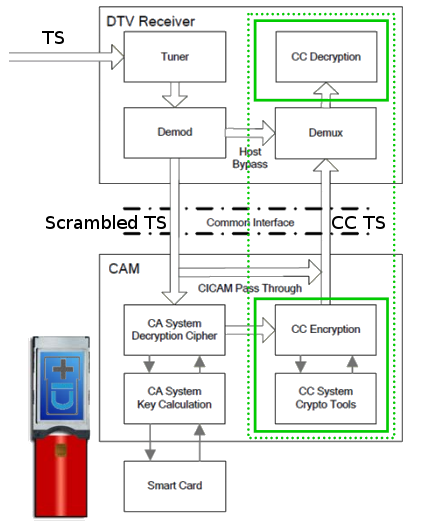
\includegraphics[width=0.5\textwidth]{CIPlus}
  \caption{CI-Plus interface. Image remade from \citep[p. 10]{CI+:2011}}
  \label{img:CIPlus}
\end{figure}

%CIPlus encoding is often used to protect HD content, but not SD content. Since HD content is more high-profile, content distributors are more tend to want to protect it than the SD content. (High Defintion, Standard Definition. HD > 720p)

\section{Conditional Access Module}\label{sec:CAM}
CA modules (CAMs) are responsible of decoding the scrambled TS 
received from the host. The CAM is often input to a PCMCIA slot 
(Personal Computer Memory International Association) either in the TV 
or the STB. The CAM consists of a slot for a smart-card and a 
descrambler. The smart card decodes the ECM and sends the CW to the 
descrambler. The TS is then descrambled and the clear TS is sent back 
to the host from the CAM.
